\chapter{Introducción al Equipo de trabajo, subcontrataciones y alianzas}
\label{cap:subdoc12}
\renewcommand{\arraystretch}{1.15}
\setlength{\tabcolsep}{4pt}
\renewcommand{\topfraction}{0.90}
\renewcommand{\textfraction}{0.08}

LafroX responde ante Distribuidora Puelche S.A. por los 230 paquetes de la estructura de descomposición del trabajo (EDT), desde el diseño hasta la salida del servicio. Para ejecutarlos dispone de 137 plazas que se activan en distintos meses del contrato. La dirección, la construcción, la implantación y la operación quedan en manos de LafroX. La intervención de terceros se limita a resultados especializados de infraestructura y seguridad; las alianzas aportan suministro y soporte de fabricante.

El Subdocumento 1, sección 1.5, define la Jefatura de Proyecto y siete ámbitos de responsabilidad; su sección 1.6 identifica las alianzas. El Subdocumento 7, secciones 7.1 y 7.2, organiza el trabajo en productos y frentes. El Formulario T-14 identifica al responsable de cada paquete y el Formulario T-15, sección 4, distribuye las horas y las plazas en el tiempo. Sobre esa base se asignan aquí los titulares que entregan la solución y los que sostienen la operación descrita en los Subdocumentos 10 y 11.

Los Anexos 12.A a 12.D contienen la matriz de asignación, los currículos, el cálculo de dedicación y los compromisos individuales. El Formulario T-8, sección 1, identifica al equipo nominado y, en su sección 2, declara las subcontrataciones y alianzas. Ambos respaldan la identificación del equipo y de la participación externa en la oferta (Bases Administrativas, Formulario T-7, Subdocumento 12, p.~59).

\section{Equipo de trabajo}

Diez titulares conducen el trabajo técnico y de gestión. El Jefe de Proyecto integra sus decisiones durante los 56 meses del contrato. La responsabilidad por un paquete, las horas que aporta un especialista y el número de personas que deben concurrir en un mes son medidas distintas: la primera determina quién responde por el resultado; las otras dos permiten programar su ejecución.

\subsection{Estructura organizacional del proyecto}

El Jefe de Proyecto reporta al Comité Ejecutivo y recibe el reporte de los responsables de los tres frentes de la Figura~\ref{fig:12-organigrama}. Dos analistas de la oficina de gestión de proyectos (PMO) apoyan a la jefatura: consolidan el avance, mantienen los acuerdos con el CLIENTE y dan seguimiento a las dependencias entre frentes.

\begin{figure}[htbp]
  \centering
  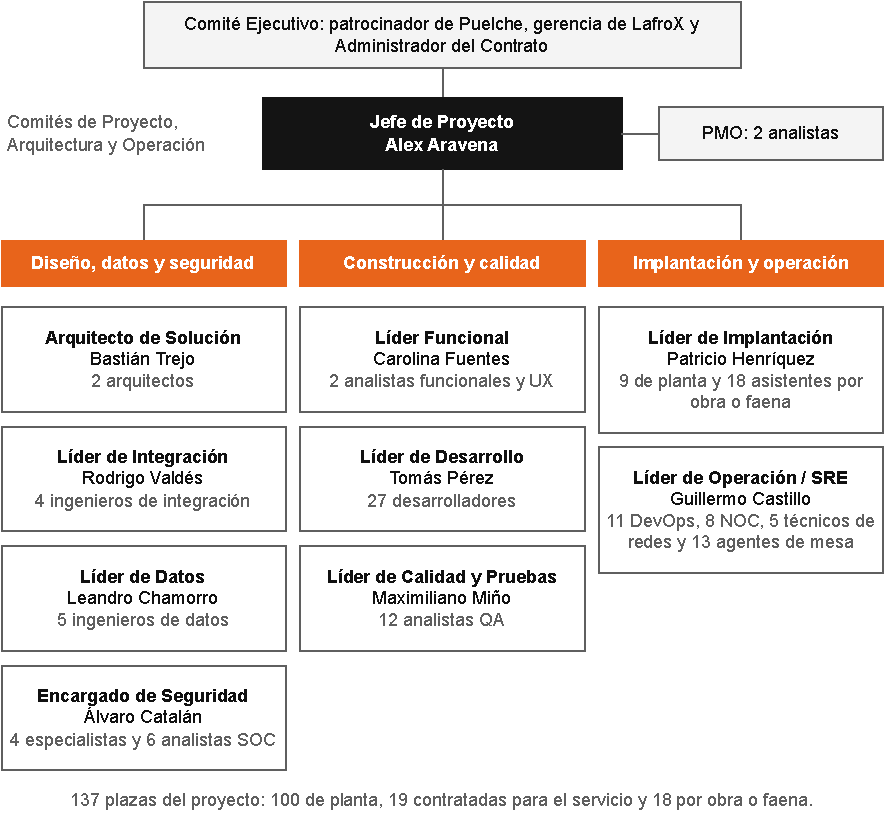
\includegraphics[width=\linewidth]{figuras/organigrama-proyecto.pdf}
  \caption{Líneas de reporte y composición de los frentes. Fuente: elaboración propia a partir del Subdocumento 1, sección 1.5, y del Formulario T-15.}
  \label{fig:12-organigrama}
\end{figure}

Las 137 plazas del organigrama no son puestos simultáneos: 100 provienen de la planta, 19 se contratan para el servicio y 18 para el despliegue en terreno. Las cifras de apoyo en las cajas se suman a cada titular, salvo cuando la figura indica que ya lo incluyen. El frente de \emph{Diseño, datos y seguridad} reúne arquitectura, integración, datos y seguridad. El Encargado de Seguridad de la Información coordina la ejecución con el Jefe de Proyecto, pero conserva la línea independiente de Seguridad del Subdocumento 1: puede elevar hallazgos sin someterlos a aprobación de Desarrollo. El frente de \emph{Construcción y calidad} vincula el análisis funcional con Desarrollo y con las pruebas de aceptación. El de \emph{Implantación y operación} conecta los equipos de terreno con el NOC, la mesa y la ingeniería de confiabilidad del servicio (SRE).

La representación de LafroX depende del tipo de decisión (Bases Administrativas, art.~71, pp.~37--38). En el \textbf{Comité Ejecutivo mensual}, el Jefe de Proyecto eleva las decisiones que comprometen al conjunto del contrato. En el \textbf{Comité de Proyecto quincenal}, la jefatura, con la PMO y los titulares de los frentes involucrados, contrasta el avance con los hitos y acuerda con el CLIENTE cómo resolver las desviaciones. En la \textbf{reunión semanal de seguimiento}, los responsables de paquetes informan los bloqueos al Jefe de Proyecto; la PMO registra la decisión o la materia que debe elevarse al comité.

El Arquitecto de Solución participa permanentemente en el \textbf{Comité de Arquitectura mensual}. El Líder de Integración y el Líder de Datos concurren cuando se deciden interfaces o migraciones; el Encargado de Seguridad de la Información integra el comité y evalúa el efecto de cada decisión sobre los controles. En el \textbf{Comité de Operación mensual}, desde el mes 13, el Líder de Operación / SRE representa al servicio junto al Encargado de Seguridad de la Información para incidentes de seguridad y al Líder de Implantación y Gestión del Cambio mientras haya despliegue en terreno. La mesa de servicio inicia su turno propio en el mes 16; en los meses 13 a 15 la representa en el comité el Líder de Operación / SRE y, desde el mes 16, el agente de ese turno que él designe en el acta. Los asuntos que exceden sus facultades vuelven al Jefe de Proyecto.

\subsection{Roles, responsabilidades y matriz de asignación}

El \textbf{Jefe de Proyecto} controla el alcance, los hitos y los compromisos con el CLIENTE. El \textbf{Arquitecto de Solución} mantiene la coherencia entre la nube y los sitios locales. El \textbf{Encargado de Seguridad de la Información} define los controles, supervisa las pruebas independientes y dirige la respuesta a incidentes de seguridad. El \textbf{Líder de Datos} responde por los modelos, las migraciones y la conciliación de los datos transferidos.

El \textbf{Líder Funcional} traduce la venta, la bodega y el reparto en requisitos y criterios de aceptación. El \textbf{Líder de Integración} especifica y prueba los intercambios con sistemas heredados. El \textbf{Líder de Desarrollo} dirige la construcción e integración de aplicaciones y servicios. El \textbf{Líder de Calidad y Pruebas} organiza las pruebas y conserva la evidencia que sustenta la aceptación.

El \textbf{Líder de Implantación y Gestión del Cambio} coordina la capacitación, la entrada por sitio y el acompañamiento a usuarios. El \textbf{Líder de Operación / SRE} habilita la plataforma y conduce el servicio, desde la atención de incidentes hasta la recuperación. La Tabla~\ref{tab:12-asignacion} distingue los productos en que cada titular responde por paquetes de aquellos en que solo aporta horas propias. P1 a P10 son los productos del Formulario T-14; sus nombres figuran en el Anexo 12.A.

\parte{tablas/tab_SD12_asignacion}

La mayor concentración corresponde al Líder de Operación / SRE: 63 paquetes, el 27,4~\% del total. De ellos, 28 corresponden al producto de infraestructura y 12 al de operación y salida. El Jefe de Proyecto concentra 24 de sus 33 paquetes en la gestión del proyecto. El Líder Funcional y el Líder de Integración no son titulares de paquetes: su trabajo se reconoce en las horas del T-15. Así, por ejemplo, la participación del Líder de Integración en P5 no transfiere la responsabilidad por los paquetes de datos migrados.

\subsection{Equipo clave nominado}

Las ocho filas fijas del Formulario T-8 constituyen el equipo clave. Cubren los seis roles habilitantes: Jefe de Proyecto, Arquitecto de Solución, Encargado de Seguridad de la Información, Líder de Datos, Líder de Calidad y Pruebas y Líder de Operación / SRE. La acreditación reúne nominación, dedicación, currículo y carta de compromiso (Bases Administrativas, art.~34, p.~22). Los ocho titulares aparecen en el video de la oferta (Bases Técnicas Transversales, RT-24.01, p.~41).

El Líder Funcional y el Líder de Integración son también roles mínimos, pero no pertenecen al equipo clave del video ni al denominador para la rotación. El Formulario T-8 los nomina bajo «Otros roles», y ambos cuentan con currículo. La Tabla~\ref{tab:12-equipo} relaciona a los diez titulares con los requisitos de su perfil (Bases Técnicas Transversales, sección 19.2, pp.~33--34). Los currículos se encuentran en el Anexo 12.B y los compromisos en el Anexo 12.D.

\parte{tablas/tab_SD12_equipo}

La dedicación declarada se expresa por fase. Para calcular la carga media imputada respecto de una jornada completa, se usan las horas del T-15. En implementación se dividen las HH del perfil por \(20 \times 128\) = 2.560 HH; en Operación, por \(36 \times 128\) = 4.608 HH (Formulario T-15, sección 4.1). Para Jefatura y Desarrollo en implementación y para SRE en Operación, el 100~\% de la tabla expresa la jornada comprometida. El Anexo 12.C concilia esa jornada con las HH que el T-15 valoriza en cada fase; el total de cada perfil en los 56 meses no cambia. Para Jefatura en Operación, 1.012,87 HH sobre 4.608 HH equivalen al 22~\% redondeado. Para el perfil 03S, las HH se distribuyen entre dos arquitectos senior antes de calcular el promedio individual (Anexo 12.C).

El compromiso mensual del Jefe de Proyecto en implementación es de 128 HH, con dedicación exclusiva y facultades para dirigir al equipo y representar a LafroX ante el CLIENTE (Bases Administrativas, art.~70.3, p.~37). El Líder de Desarrollo y el Líder Funcional también tienen jornada completa en todos los meses de implementación. El Arquitecto de Solución concentra su dedicación en el diseño de los meses 1 a 7 y mantiene su asiento en el Comité de Arquitectura hasta el mes 56.

El Encargado de Seguridad de la Información y el Líder de Calidad y Pruebas mantienen participación durante ambas fases. El Líder de Datos y el Líder de Integración tienen horas en todos los meses de implementación y apoyo puntual en Operación. El Líder de Operación / SRE participa desde el mes 1, antes del mínimo del mes 6, y asume como gerente de servicio con jornada completa del mes 21 al 56. El Líder de Implantación y Gestión del Cambio también participa desde el mes 1, antes del mínimo del mes 8; concentra su trabajo en las marchas blancas y el cierre, entre los meses 13 y 22.

Con febrero de 2027 como mes 1, vencen durante el primer año la CISSP de Álvaro Catalán y la CSM de Alex Aravena. En 2028 vencen la PMP de Alex Aravena, la credencial de arquitectura AWS de Bastián Trejo (marzo, mes 14), las de ITIL de Guillermo Castillo (junio, mes 17) y la de desarrollo AWS de Tomás Pérez (septiembre, mes 20). La credencial de datos AWS de Leandro Chamorro vence en abril de 2029, mes 27. La CSCP de Carolina Fuentes está vigente hasta 2030, después de su participación. Las credenciales ISTQB no vencen y la de Prosci no requiere renovación periódica.

\subsection{Curva de dotación por fase}

El máximo simultáneo es de 58 plazas, no de 137. El Formulario T-15, sección 4, convierte las horas de cada grupo de origen en personas por mes: \(\mathrm{plazas}=\lceil\mathrm{HH~del~grupo~en~el~mes}/128\rceil\). Se redondea cada grupo hacia arriba antes de sumar: una fracción de jornada de redes no cubre una fracción vacante en implantación. La Figura~\ref{fig:12-curva} agrupa la demanda mensual para mostrar cuándo coinciden construcción, despliegue y servicio.

\begin{figure}[htbp]
  \centering
  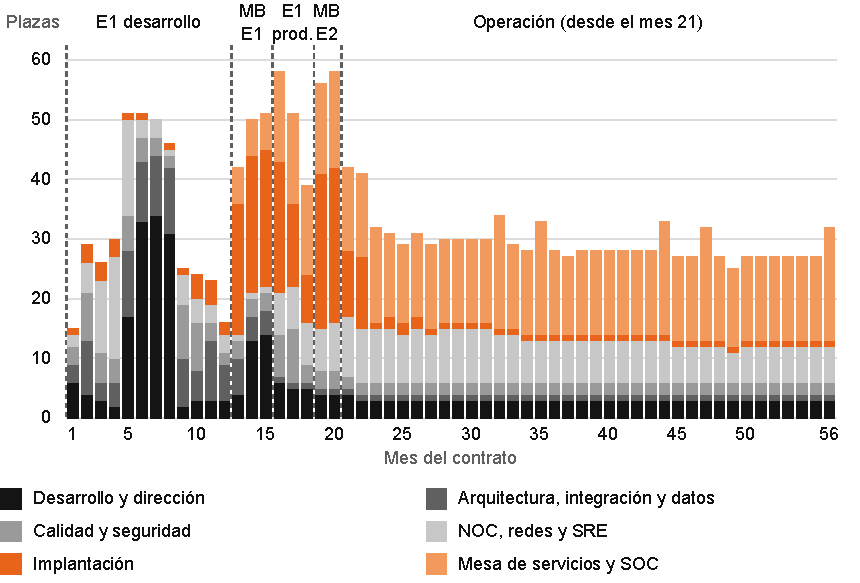
\includegraphics[width=\linewidth]{figuras/curva-dotacion.pdf}
  \caption{Demanda mensual de plazas durante el contrato. Fuente: elaboración propia a partir del Formulario T-15, sección 4, demanda mensual de plazas por grupo de origen.}
  \label{fig:12-curva}
\end{figure}

La Etapa 1 alcanza 51 plazas tanto en el mes 5 como en el 6. En el primero, SRE ocupa sus 12 plazas y, en el segundo, Desarrollo llega a 33. El máximo propio de Desarrollo, 34 plazas en el mes 7, no coincide con ese máximo conjunto. En el mes 16 la Etapa 1 entra en producción mientras continúa el desarrollo de la Etapa 2; en el mes 20 la segunda marcha blanca concentra el apoyo a usuarios. Ambos meses demandan 58 plazas, pero no la misma combinación de perfiles. La Tabla~\ref{tab:12-fases} separa el cierre de la Etapa 2 de los restantes meses de Operación para no diluir el esfuerzo de terreno en el promedio.

\parte{tablas/tab_SD12_fases}

La Operación contractual comienza en el mes 21. Al concluir el cierre de la Etapa 2, la demanda baja a unas 29 plazas en promedio. El refuerzo estacional recae en la mesa, que llega a 13 agentes en los meses 32, 35, 44, 47 y 56, sin ampliar la dotación del SOC.

La tabla «Plazas previstas y demanda máxima mensual por origen» del Formulario T-15 contrasta estas demandas con la planta del Subdocumento 1, tabla 1.3. Desarrollo llega a 34 de 48; Arquitectura e integración, a 11 de 15; NOC y redes, a 8 de 32; SRE y nube, a 12 de 12; Calidad, a 8 de 10, y Seguridad, a 5 de 7. Esta comparación es por origen contractual, no por caja del organigrama. Las 100 plazas de planta incluyen 91 de los grupos técnicos y 9 de Implantación. En terreno, las 18 plazas por obra o faena elevan la disponibilidad a 27 frente a una demanda máxima de 26. Las 19 plazas del servicio se contratan fuera de la planta: 13 de mesa y 6 del SOC. Para la campaña de Calidad del 25 de octubre al 11 de noviembre de 2027, el SD9 prevé 13 personas durante 13 días hábiles: el líder y nueve analistas QA senior del grupo Calidad, más tres analistas QA junior de origen Desarrollo (T-15, perfiles 16, 19S y 19J). El máximo mensual de ocho plazas mide las horas del grupo Calidad. El Líder de Calidad y Pruebas confirma en el registro de turnos la disponibilidad de cada persona antes de reservar la sesión. A 6,4 HH netas por persona y día, las trece cubren 82,9 HH diarias de demanda con 83,2 HH de capacidad (T-13, sección 8.3). Los tres refuerzos ya están incluidos en las 137 plazas.

\subsection{Gestión del conocimiento, retención y continuidad}

Cada titular comparte con su suplente las decisiones y los procedimientos que permiten continuar su trabajo. La Tabla~\ref{tab:12-suplentes} identifica el perfil que se prepara junto al titular; la suplencia operativa no autoriza por sí sola un cambio en la nómina contractual.

\parte{tablas/tab_SD12_suplentes}

Los diez suplentes provienen del mismo grupo de origen del titular y ya forman parte de las plazas del T-15, por lo que una ausencia temporal se cubre sin incorporar personal externo. La suplencia no sustituye la autorización previa y escrita que exige un cambio de titular (Bases Administrativas, art.~76.1, p.~39).

El Anexo 8.H del SD8 programa las 160 HH de reserva de gestión en cuatro ciclos de 40 HH, en los meses 12, 18, 24 y 40. En el primer turno de los meses 12 y 18, un analista PMO cubre ocho horas delegables de Jefatura. En el primer turno de los meses 24 y 40, un profesional DevOps habilitado cubre ocho horas operativas de SRE. La reserva de gestión queda fuera de la línea base. Las 3.072 HH protegidas para correcciones de la Etapa 1 ya integran la línea base del T-15.

La PMO puede sostener el seguimiento de hitos y acuerdos durante una ausencia de la jefatura, pero no sustituye sus facultades ante el CLIENTE. Para un reemplazo formal, LafroX solicita autorización previa y escrita, presenta un perfil igual o superior y asegura al menos 15 días hábiles de traslape sin costo para el CLIENTE (Bases Administrativas, arts.~76.1 y 76.2, p.~39).

El límite de rotación del 30~\% en 12 meses se aplica sobre ocho titulares: \(0{,}30 \times 8 = 2{,}4\), de modo que caben como máximo dos reemplazos, ambos autorizados (Bases Administrativas, art.~76.3, p.~39). LafroX procura evitar todo reemplazo no planificado e informa al Comité Ejecutivo desde el primero. Un reemplazo no autorizado constituye incumplimiento aunque no se alcance el límite y da lugar a la multa por persona reemplazada (Bases Administrativas, art.~80, p.~41).

El conocimiento queda distribuido entre titular, suplente y equipo, no solo en la memoria de quien ocupa el cargo (Bases Administrativas, art.~76.4, p.~39). El espacio colaborativo accesible al CLIENTE permite consultar acuerdos, decisiones de diseño y procedimientos vigentes (Bases Técnicas Transversales, RT-19.05, p.~33). El Jefe de QA administra el repositorio corporativo de arquitectura, estándares, despliegue y recuperación; los incidentes P1 y P2 cierran con un informe \emph{post-mortem} aprobado y publicado. Los talleres trimestrales de traspaso y la revisión semestral del Comité de Calidad mantienen ese material en uso (Subdocumento 1, sección 1.3).

El T-15 imputa al paquete 9.3.1 las 1.851 HH de NOC y Mesa de mayo completo. Del 1 al 16 de mayo (384 HH de NOC y 574 HH de Mesa), mientras la Contraparte revisa el expediente de cierre de la marcha blanca entregado el 2 de mayo, ambos servicios mantienen la atención a los usuarios y alistan las colas, los turnos y los escalamientos del corte. Desde el corte nominal del 17 de mayo de 2028 (893 HH hasta el 31) sostienen la operación en producción de la Etapa 1. Del 1 al 17 de octubre, NOC, Mesa y SOC cubren ambos alcances bajo el Líder de Operación / SRE (10.1.1, 10.1.2 y 10.1.4). El corte nominal de E2 se programa para el 18 de octubre de 2028. En cada relevo de NOC, Mesa y SOC, el operador o analista saliente entrega al entrante de su servicio el turno, los tickets e incidentes abiertos, las prioridades, las dependencias, las próximas acciones y el estado de las colas. El entrante registra la recepción y conserva el reloj original de atención. El Líder de Operación / SRE coordina los relevos y el Encargado de Seguridad supervisa el del SOC (SD10, sección 10.1, y Formulario T-18).

Como parte del traspaso técnico del mes 21, el Líder de Desarrollo entrega al Líder de Operación / SRE las versiones en servicio, los procedimientos de despliegue y recuperación y los antecedentes de incidentes. Operación utiliza esos mismos procedimientos para atender el servicio mientras Implantación completa el cierre en terreno. Para retener las competencias acreditadas, LafroX inicia la renovación de cada credencial sujeta a vencimiento 60 días antes, mediante su programa corporativo de formación.

Los turnos de la mesa incorporan a los agentes de refuerzo en los meses de mayor demanda y utilizan la misma base de conocimiento que los turnos regulares. LafroX contrata al personal del SOC antes del mes 13 y mantiene seis analistas desde ese mes hasta el término del contrato. En Talca y Concepción, los 18 asistentes de implantación contratados por obra o faena reciben formación en el puesto; su participación finaliza de manera escalonada según la adopción, entre el despliegue y el cierre de los meses 13 a 22.

\section{Subcontrataciones}

LafroX ejecuta el núcleo del proyecto con personal propio, incluidas las contrataciones directas de mesa, SOC y terreno. La Tabla~\ref{tab:12-hacer-comprar} distingue qué capacidades conserva, cuáles compra como servicio estándar y en qué casos contrata un resultado especializado (Bases Administrativas, art.~73.2, p.~38).

\parte{tablas/tab_SD12_hacer_comprar}

El criterio es quién ejecuta el trabajo. AWS, CrowdStrike e Intune suministran nube, protección de equipos y gestión de dispositivos; Telsur (Grupo Gtd), Entel, Claro, Starlink e Iridium suministran conectividad. Los servicios de mapas, mensajería, pagos y custodia de respaldos y fuentes también son compras estándar: sus proveedores no ejecutan paquetes con personal propio. En cambio, la Tabla~\ref{tab:12-subcontratos} identifica los resultados que un especialista externo debe entregar y el titular que los acepta por LafroX.

\parte{tablas/tab_SD12_subcontratos}

Los siete servicios suman 1.324,80 HH externas. En los paquetes 8.3.2, 8.3.3 y 8.3.4, cada especialista aporta 128 HH; las 32 HH adicionales de técnicos de LafroX por paquete no son subcontratación. Las horas de revisión en Operación son totales del período, no horas por visita. Medida sobre las HH de la línea base, la participación conjunta de los siete servicios es del 0,65~\%, muy por debajo del tope contractual del 40~\%. Para cada adjudicación, LafroX selecciona la empresa mediante tres cotizaciones y obtiene autorización previa y escrita del CLIENTE antes de contratar (Bases Administrativas, art.~73.1, p.~38).

El responsable de cada paquete supervisa al tercero y verifica el resultado con los criterios de aceptación del T-14. Las pruebas de seguridad ofensiva quedan en manos del tercero independiente; el Líder de Desarrollo no certifica su propio trabajo. LafroX conserva la responsabilidad solidaria y aplica al subcontratista los mismos estándares de ejecución y confidencialidad (Bases Administrativas, art.~73.3, p.~38). Cada subcontratista firma un acuerdo de confidencialidad. Por su acceso a datos, el tercero de pruebas también se declara, se audita y suscribe el acuerdo de tratamiento. También se declaran y quedan sujetos a acuerdo de tratamiento los proveedores con acceso a datos del CLIENTE: AWS, CrowdStrike, Intune y custodia (Bases Administrativas, art.~73.4, p.~38; Ley 21.719).

\section{Alianzas}

Las cuatro alianzas del Subdocumento 1, sección 1.6, tienen un 0~\% de participación en la ejecución. Su aporte es el suministro y el soporte de fabricante. El CLIENTE mantiene un único canal de responsabilidad: LafroX verifica el componente recibido, gestiona los incidentes y recurre al fabricante como último nivel de escalamiento.

\textbf{AWS Partner Network.} El SD1, sección 1.6, declara la categoría Advanced Tier Services, con competencias DevOps y Migración. Esa categoría sustenta el habilitante «Capacidad de proveedor de nube» (Bases Administrativas, art.~34.1, p.~22). AWS aporta revisión Well-Architected del diseño y soporte empresarial; el Arquitecto de Solución conserva la decisión de diseño. La alianza vence en marzo de 2027, mes 2. Arquitectura y Operación inician la renovación en diciembre de 2026, más de 60 días antes del vencimiento.

\textbf{Zebra Technologies.} La categoría Premier Solution Partner respalda la garantía y el soporte de fábrica de terminales móviles, lectores e impresoras. El CLIENTE compra esos equipos sobre la especificación que LafroX entrega en el paquete 8.1.1. La alianza vence en junio de 2027, mes 5.

\textbf{Fortinet / Cisco.} La categoría Select Partner cubre el suministro y el soporte de los firewalls FortiGate y los switches Cisco adquiridos por LafroX. La instalación y la operación de red siguen a cargo de sus técnicos. La alianza vence en septiembre de 2027, mes 8.

\textbf{Starlink Business.} La condición Authorized Enterprise Reseller respalda los terminales satelitales de los cinco sitios. El fabricante atiende el escalamiento relativo al terminal; LafroX responde por la conectividad del servicio ante el CLIENTE. La alianza vence en diciembre de 2027, mes 11.

Las cuatro alianzas vencen durante el primer año contractual. El Líder de Operación / SRE y el Arquitecto de Solución inician cada gestión 60 días antes del vencimiento, con inicio previo al mes 1 en el caso de AWS, y conservan la evidencia de vigencia para el CLIENTE. Renovar una alianza no cambia la asignación de paquetes ni incorpora personal del fabricante al equipo de ejecución.

\section*{Referencias}
\phantomsection
\addcontentsline{toc}{section}{Referencias}

Las condiciones contractuales y los requisitos técnicos citados corresponden a los siguientes documentos de la licitación:

\begin{itemize}
\item Distribuidora Puelche S.A. (2026a). \emph{Bases Administrativas}.
\item Distribuidora Puelche S.A. (2026b). \emph{Bases Técnicas Transversales}.
\item Ley N.° 21.719. (2024). \emph{Regula la protección y el tratamiento de los datos personales y crea la Agencia de Protección de Datos Personales}. Diario Oficial de la República de Chile.
\end{itemize}

\begin{anexohorizontal}
\setlength{\textwidth}{\linewidth}
\section*{Declaración de uso de IA}
\phantomsection
\addcontentsline{toc}{section}{Declaración de uso de IA}

La Tabla~\ref{tab:12-ia} identifica el uso de herramientas y el alcance de la revisión humana por pieza de la oferta.

\parte{tablas/tab_SD12_IA}

El uso en diagramas se limita al organigrama y a la curva de dotación de la sección 12.1.
\end{anexohorizontal}
